\chapter*{Appendix: Research Paper: YOLOv11n-MobileNetV4 for Edge AI in Adaptive AUTOSAR}
\phantomsection
\label{chap:append}

\addcontentsline{toc}{chapter}{Appendix: Research Paper}

Following the successful completion of the project, a comprehensive research paper was submitted to the IEEE Sensors Applications Symposium (SAS) 2026, focusing on Edge AI. The manuscript presents a lightweight framework for real-time traffic light detection, seamlessly integrated into the AUTOSAR Adaptive Platform for ADAS applications.

To address the strict latency and resource constraints of edge sensor nodes, the paper proposes a highly optimized YOLO11-MobileNetV4 architecture using post-training quantization for efficient CPU-only inference. Implemented as an SOA-compliant C++ Adaptive Application, the pipeline proves the viability of accelerator-free edge computing. Experimental results demonstrate that the proposed model achieves a real-time throughput of approximately 27 frames per second at an input resolution of $320 \times 320$ on standard embedded hardware. It delivers a 2.5$\times$ speedup over the YOLO11n baseline and outperforms YOLO8n and SSD-MobileNetV3 in inference speed, while maintaining superior accuracy (mAP@50) compared to the SSD baseline.

The original manuscript for this IEEE submission is appended below, serving as a formal academic validation of the proposed ADAS development methodology.

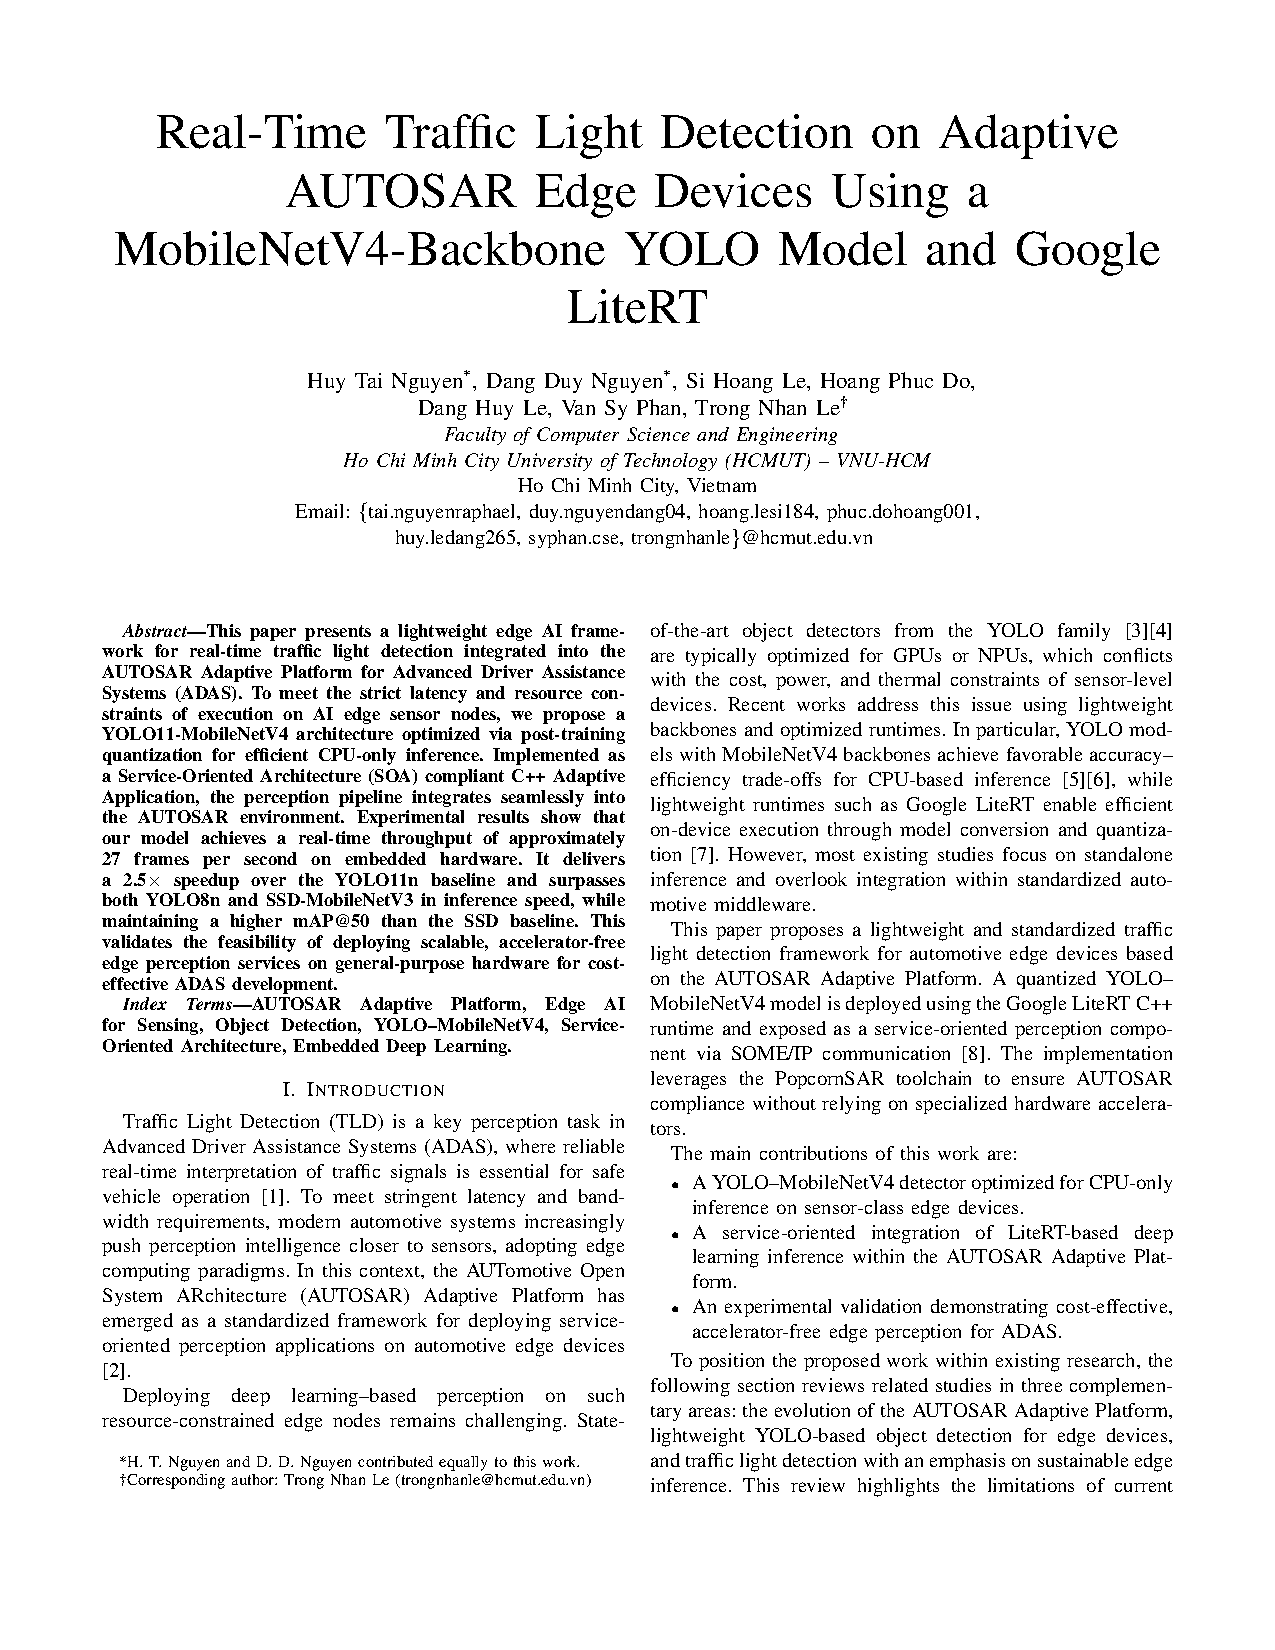
\includepdf[pages=-, scale=0.85, pagecommand={}]{YOLO_MobilenetV4_LiteRT_AUTOSAR_paper.pdf}
